
% Lecture Notes: Sequence Modeling with Hidden Markov Models (HMMs)

\section{Introduction and Biological Motivation}

When analyzing newly sequenced and assembled genomes, we are typically presented with large, unlabelled chunks of DNA. Our primary goal is genome annotation: finding functionally relevant regions such as protein-coding genes, regulatory motifs, and promoters within a vast sea of non-coding nucleotides. This is challenging because biological data is inherently noisy due to natural variation, evolutionary mutation, and sequencing errors, making rigid, deterministic rules brittle.

While simpler models like sequence alignment profiles or position weight matrices (PWMs) are useful for identifying fixed-length patterns (e.g., transcription factor binding sites), they fall short when modeling more complex genomic structures.

\begin{important}
  \textbf{Property: Variable Length of Genomic Elements} \\
  Many functional genomic elements have highly variable lengths. For example, a protein-coding gene consists of an initial sequence (\textit{ATG}), an unspecified number of codons (triplets), separated by variable-length non-coding introns, and concluding with a stop codon (\textit{TGA}, \textit{TAA}, or \textit{TAG}). Fixed-length motifs cannot accurately model these features.
\end{important}

\subsection{Goals of Sequence Modeling}
By modeling DNA sequences probabilistically, we achieve three primary objectives:
\begin{itemize}
    \item \textbf{Generative Simulation}: The ability to emit or generate random DNA sequences of a specific type (e.g., simulating promoters) that preserve the statistical properties of that type, even if they do not identically match any known sequence.
    \item \textbf{Sequence Recognition (Decoding)}: The ability to analyze an unlabelled sequence and infer the hidden state (e.g., coding vs. non-coding) that was most likely to have generated the observed nucleotides.
    \item \textbf{Feature Learning}: The ability to train generative models on large datasets to automatically learn the distinguishing sequence characteristics of different genomic states.
\end{itemize}

\section{Markov Chains and Hidden Markov Models}

Probabilistic sequence modeling assigns ``degrees of belief'' to our classifications. At the foundation of these methods are Markov Chains, named after the Russian mathematician Andrey Markov, who formalized stochastic processes that transition from one state to another.

\subsection{Markov Chains}

A Markov Chain is a system that models sequences of directly observable data items (e.g., symbols or letters).

\begin{important}
  \textbf{Definition (Markov Chain):} A triplet \( (Q, p, A) \), where:
  \begin{itemize}
      \item \( Q \) is a finite set of observable states (corresponding to a symbol alphabet \( \Sigma \)).
      \item \( p \) is a vector of initial state probabilities.
      \item \( A \) is the transition probability matrix, where \( a_{kl} = P(x_i = l \mid x_{i-1} = k) \).
  \end{itemize}
\end{important}

\sta The defining feature of a Markov Chain is that it is \textbf{memoryless} (the Markov property). The probability of transitioning to the next state depends \textit{only} on the current state, completely ignoring the historical path taken to arrive there:
\begin{equation}
P(x_i \mid x_{i-1}, \dots, x_1) = P(x_i \mid x_{i-1})
\end{equation}

The probability of observing a specific sequence \( x \) of length \( L \) is computed by multiplying the initial probability and all subsequent sequential transition probabilities:
\begin{equation}
P(x) = P(x_1) \times \prod_{i=2}^{L} P(x_i \mid x_{i-1})
\end{equation}

\textbf{Example:} Predicting tomorrow's weather.
If the states (Sunny, Rainy, Cloudy) are directly observable, we can measure the probability that a sunny day is followed by a rainy day. There are no hidden variables; what you see is what you get.

\subsection{Hidden Markov Models (HMMs)}

In biological applications, the functional ``state'' of the genome (e.g., whether a region is an exon or an intron) is not explicitly written in the sequence. We only observe the emitted sequence of nucleotides (\(A, C, G, T\)). This requires a Hidden Markov Model.

\begin{important}
  \textbf{Definition (Hidden Markov Model):} A 5-tuple \( (Q, V, p, A, E) \), where:
  \begin{itemize}
      \item \( Q \) is a finite set of hidden states \( q_n \); \( |Q| = N \).
      \item \( V \) is a finite set of observable symbols \( v_m \); \( |V| = M \).
      \item \( p \) is a vector of initial state probabilities.
      \item \( A \) is the matrix of state transition probabilities: \( a_{kl} = P(\pi_i = l \mid \pi_{i-1} = k) \).
      \item \( E \) is the emission probability matrix: \( e_k(v_m) = P(x_i = v_m \mid \pi_i = k) \).
  \end{itemize}
\end{important}

\sta In an HMM, \textbf{both} state transitions and symbol emissions are memoryless. The emitted symbol \( x_i \) depends \textit{only} on the current hidden state \( \pi_i \), and the next state \( \pi_{i+1} \) depends \textit{only} on \( \pi_i \). We use Bayes' rule to infer the hidden state given the observed symbol.

% [IMAGE: Side-by-side comparison. Left side shows a Markov Chain of weather (Sun, Clouds, Rain, Snow) transitioning directly between each other. Right side shows an HMM where hidden states (Summer, Winter) transition between each other, and each hidden state emits observable weather symbols with specific probabilities.]
\myimage{7_1/1.png}{Side-by-side comparison. Left side shows a Markov Chain of weather (Sun, Clouds, Rain, Snow) transitioning directly between each other. Right side shows an HMM where hidden states (Summer, Winter) transition between each other, and each hidden state emits observable weather symbols with specific probabilities.}

\textbf{Example:} Seasons and Weather.
Consider seasons (Summer, Winter) as the hidden states \( Q \) and the weather (Sunny, Snow) as the observable symbols \( V \). We cannot directly observe the season, but we can deduce it because the hidden state heavily influences the emission probabilities.

\subsection{The Dishonest Casino Example}

To understand how we extract signal from noise with an HMM, consider a casino that uses two dice:
\begin{itemize}
    \item \textbf{Fair die (\(D_F\)):} \( P(1..6) = \frac{1}{6} \)
    \item \textbf{Loaded die (\(D_L\)):} \( P(6) = \frac{1}{2} \), and \( P(1..5) = \frac{1}{10} \)
\end{itemize}
The casino player switches between the fair and loaded die on average once every 20 turns. Thus, the transition probabilities are \( a_{FL} = 0.05 \) and \( a_{FF} = 0.95 \).

\begin{center}
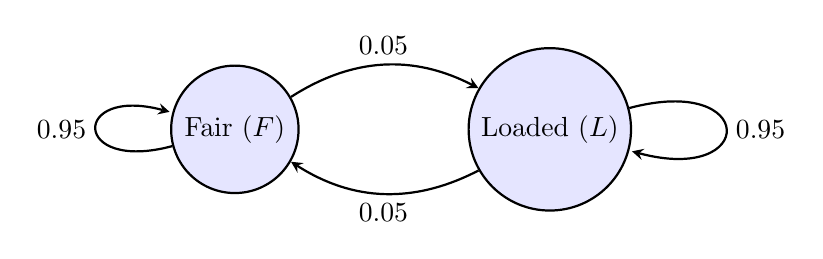
\begin{tikzpicture}[->, >=stealth, auto, node distance=4cm, thick, state/.style={circle, draw, minimum size=1.5cm, fill=blue!10}]
\node[state] (F) {Fair ($F$)};
\node[state] (L) [right of=F] {Loaded ($L$)};

\path
(F) edge [loop left] node {\(0.95\)} (F)
    edge [bend left] node {\(0.05\)} (L)
(L) edge [loop right] node {\(0.95\)} (L)
    edge [bend left] node {\(0.05\)} (F);
\end{tikzpicture}
\end{center}

We observe a sequence of die rolls (the emissions) but do not know which die the dealer is using (the hidden path). Our goal is to determine when the dealer is using the loaded die. 

\textbf{Example: The Dishonest Genome}\\
This maps directly to genomics. A genome might randomly transition between human DNA (Background) and integrated viral DNA. The observable alphabet is $\{A, C, G, T\}$. Viral DNA and Human DNA will have distinct emission probabilities for these nucleotides (e.g., varying GC-content), and transitions between them are rare but possible.

% [IMAGE: Header of the paper 'Prediction of Complete Gene Structures in Human Genomic DNA' by Burge and Karlin, introducing GENSCAN.]
\myimage{7_1/2.png}{Header of the paper 'Prediction of Complete Gene Structures in Human Genomic DNA' by Burge and Karlin, introducing GENSCAN.}
% [IMAGE: Complex HMM architecture (GENSCAN) for predicting protein-coding genes, showing hidden states for UTRs, Exons, Introns, and start/stop/splice signals across different reading frames.]

\section{The Six Algorithmic Settings for HMMs}

When working with HMMs, we address three main types of problems, each under two different constraints (evaluating a single specific path vs. evaluating all possible paths):

\begin{table}[h]
\centering
\begin{tabularx}{\textwidth}{l X X}
\toprule
\textbf{Task} & \textbf{One Path (Optimal)} & \textbf{All Paths (Summed)} \\
\midrule
\textbf{Evaluation} & 1. Scoring $x$ over the optimal path. & 2. Scoring $x$ over all paths (Forward algorithm). \\
\textbf{Decoding} & 3. Finding the best state sequence (Viterbi algorithm). & 4. Probabilistic label per position (Posterior decoding). \\
\textbf{Learning} & 5a. Supervised MLE (if labels known). \newline 5b. Viterbi training (if labels unknown). & 6. Baum-Welch / EM (if labels unknown). \\
\bottomrule
\end{tabularx}
\caption{The six algorithmic settings for handling HMMs in sequence analysis.}
\end{table}

\subsection{Evaluation: Scoring a Sequence}

\subsubsection{Setting 1: Scoring a Single Path (Joint Probability)}

If we are given an exact sequence of observations \( x \) and a specifically assumed hidden path \( \pi \), we calculate their joint probability by multiplying the transition probabilities along the path by the emission probabilities at each step:

\[ P(x, \pi) = P(x \mid \pi) P(\pi) = p(\pi_1) e_{\pi_1}(x_1) \prod_{i=1}^{N-1} a_{\pi_i \pi_{i+1}} e_{\pi_{i+1}}(x_{i+1}) \]

\textbf{Example:} Comparing paths in the Dishonest Casino.\\
Assume we observe the sequence \( x = 1, 2, 1, 5, 6, 2, 1, 6, 2, 4 \). Assuming an initial probability of 0.5 for starting in either state:
\begin{itemize}
    \item \textbf{All-Fair path (\(\pi = F, \dots, F\)):}
    \[ P(x, \text{all-Fair}) = 0.5 \times \left(\frac{1}{6}\right)^{10} \times (0.95)^9 \approx 5.2 \times 10^{-9} \]
    \item \textbf{All-Loaded path (\(\pi = L, \dots, L\)):}
    \[ P(x, \text{all-Loaded}) = 0.5 \times \left(\frac{1}{10}\right)^8 \times \left(\frac{1}{2}\right)^2 \times (0.95)^9 \approx 7.9 \times 10^{-10} \]
\end{itemize}
The all-Fair path is about 6.59 times more likely than the all-Loaded path for this particular sequence. 
\sta \textit{Note:} Joint probabilities approach zero rapidly, necessitating the use of log-scores to prevent computational underflow.

% INSERT /home/papagna/Projects/latex_bio/lex_md/07-Sequence_modeling-HMM_07-Sequence_modeling-HMM/imgs/cropped_page27_idx20.jpg

\subsubsection{Setting 2: Scoring All Paths (Forward Algorithm)}

To find the \textit{total} probability \( P(x) \) that the model generated the sequence, regardless of the specific path taken, we sum the joint probabilities over an exponential number of possible paths:
\[ P(x) = \sum_{\pi} P(x, \pi) \]

% INSERT /home/papagna/Projects/latex_bio/lex_md/07-Sequence_modeling-HMM_07-Sequence_modeling-HMM/imgs/cropped_page42_idx34.jpg

We compute this efficiently in $\mathcal{O}(K^2 N)$ time using dynamic programming via the \textbf{Forward Algorithm}. Let \( f_k(i) \) be the probability of generating the prefix sequence \( x_1 \dots x_i \) and ending in state \( k \).

\begin{itemize}
    \item \textbf{Initialization:} \( f_0(0) = 1 \), \( f_k(0) = 0 \) for all \( k > 0 \).
    \item \textbf{Iteration:} 
    \[ f_k(i) = e_k(x_i) \times \sum_j \left( a_{jk} f_j(i-1) \right) \]
    \item \textbf{Termination:} The total probability of the sequence is \( P(x) = \sum_k f_k(N) \).
\end{itemize}

% INSERT /home/papagna/Projects/latex_bio/insert/screenshot-2026-06-10_23-40-59.png

\subsection{Decoding: Finding the Hidden States}

\subsubsection{Setting 3: Decoding the Most Likely Path (Viterbi Algorithm)}

Given only the observed emissions \( x \), we usually want to find the single most likely sequence of hidden states \( \pi^* \) that generated it. The problem exhibits \textit{optimal substructure}: the best path reaching state $k$ at step $i$ is composed of the best path reaching some state $j$ at step $i-1$, followed by the optimal transition to $k$.

\begin{important}
  \textbf{Viterbi Algorithm:} A dynamic programming algorithm that computes the most likely sequence of hidden states. Let \( V_k(i) \) be the probability of the most likely path generating sequence $x_1 \dots x_i$ and ending in state $k$.
  \begin{itemize}
      \item \textbf{Initialization:} \( V_0(0) = 1 \); \( V_k(0) = 0 \) for all \( k > 0 \).
      \item \textbf{Iteration:} \( V_k(i) = e_k(x_i) \times \max_j (a_{jk} V_j(i-1)) \)
      \item \textbf{Termination:} \( P(x, \pi^*) = \max_k V_k(N) \)
  \end{itemize}
\end{important}

We keep pointers to the maximizing state \( j \) at each step to reconstruct the optimal path \(\pi^*\) via traceback. The time complexity is $\mathcal{O}(K^2N)$ and space complexity is $\mathcal{O}(KN)$.

\begin{minted}{python}
# [pseudocode]
def viterbi(obs, states, init_p, trans_p, emit_p):
    V = [{}] # DP matrix
    path = {}
    
    # Initialization
    for y in states:
        V[0][y] = init_p[y] * emit_p[y][obs[0]]
        path[y] = [y]
        
    # Iteration
    for t in range(1, len(obs)):
        V.append({})
        newpath = {}
        for y in states:
            (prob, state) = max((V[t-1][y0] * trans_p[y0][y] * emit_p[y][obs[t]], y0) 
                                for y0 in states)
            V[t][y] = prob
            newpath[y] = path[state] + [y]
        path = newpath
        
    # Termination
    (prob, state) = max((V[len(obs) - 1][y], y) for y in states)
    return prob, path[state]
\end{minted}

% INSERT /home/papagna/Projects/latex_bio/insert/screenshot-2026-06-10_23-36-23.png

% INSERT /home/papagna/Projects/latex_bio/insert/screenshot-2026-06-10_23-37-16.png

\textbf{Example: Viterbi Trace for a Viral (V) vs. Self (S) Genome Model} \\
Assume we observe the sequence \( x = (G, C, G, A, T) \).
Initial: \( p_V = 0.5, p_S = 0.5 \). \\
Transitions: \( a_{VV} = 0.15, a_{VS} = 0.85, a_{SV} = 0.05, a_{SS} = 0.95 \). \\
Emissions \( V \): \( G(0.33), C(0.33), A(0.17), T(0.17) \). \\
Emissions \( S \): \( G(0.25), C(0.25), A(0.25), T(0.25) \).

\begin{enumerate}
    \item \textbf{Initialization \( i=1 \) (Emission 'G'):}
    \( V_V(1) = 0.5 \times 0.33 = 0.165 \) \\
    \( V_S(1) = 0.5 \times 0.25 = 0.125 \)
    \item \textbf{Iteration \( i=2 \) (Emission 'C'):}
    \( V_V(2) = 0.33 \times \max(0.15 \times 0.165, 0.05 \times 0.125) \approx 8.17 \times 10^{-3} \) (from V). \\
    \( V_S(2) = 0.25 \times \max(0.85 \times 0.165, 0.95 \times 0.125) \approx 3.5 \times 10^{-2} \) (from V).
    \item \textbf{Termination \& Traceback:} Continuing to \( i=5 \), the highest probability ends in state \( S \). Tracing the max pointers backwards reveals the optimal path: \( V \to S \to S \to S \to S \). 
\end{enumerate}
This demonstrates how the high transition probability from Viral to Self (\(0.85\)) dominates, making it optimal to start in the viral state but immediately switch to the self state.

% INSERT /home/papagna/Projects/latex_bio/insert/screenshot-2026-06-10_23-38-12.png

\subsubsection{Setting 4: Decoding All Paths (Posterior Decoding)}

Viterbi gives the single best path, but it ignores the probability mass of all other valid paths. To find the most likely state for a \textit{specific position} \( i \) averaged over all paths, we use \textbf{Posterior Decoding}.

% INSERT /home/papagna/Projects/latex_bio/lex_md/07-Sequence_modeling-HMM_07-Sequence_modeling-HMM/imgs/cropped_page64_idx60.jpg

We combine the \textbf{Forward algorithm} (how we got to position \( i \)) and the \textbf{Backward algorithm} (the probability of observing the remainder of the sequence given we are at state \( k \) at position \( i \)).

\textbf{The Backward Algorithm:}
Define \( b_k(i) = P(x_{i+1} \dots x_N \mid \pi_i = k) \).
\begin{itemize}
    \item \textbf{Initialization:} \( b_k(N) = a_{k0} \) (or 1 if end state transitions are uniform) for all \( k \).
    \item \textbf{Iteration:} (Working backwards from \( N-1 \) down to 1):
    \[ b_k(i) = \sum_l \left( e_l(x_{i+1}) \cdot a_{kl} \cdot b_l(i+1) \right) \]
\end{itemize}

% INSERT /home/papagna/Projects/latex_bio/insert/screenshot-2026-06-10_23-45-13.png

By multiplying the forward and backward probabilities, we isolate the probability of being in state \( k \) at position \( i \) given the entire sequence \( x \):
\[ P(\pi_i = k \mid x) = \frac{f_k(i) \cdot b_k(i)}{P(x)} \]
where \( P(x) \) can be found via the Forward algorithm, or computed as \( P(x) = \sum_l a_{0l} e_l(x_1) b_l(1) \).

\sta Posterior decoding provides the highest-confidence state at each independent position. However, because it optimizes locally, the resulting sequence of states might contain structurally impossible transitions (e.g., jumping from a Promoter directly to an Intron).

\subsection{Learning: Training HMM Parameters}

Before an HMM can decode a genome, we must estimate its parameters: transition probabilities (\( a_{kl} \)) and emission probabilities (\( e_k(x) \)).

% INSERT /home/papagna/Projects/latex_bio/insert/screenshot-2026-06-10_23-49-03.png

\subsubsection{Setting 5a: Supervised Learning (Known Labels - When the right answer is known)}

When we have training data fully annotated with true hidden states, learning uses Maximum Likelihood Estimation (MLE) by simply counting frequencies:
\[ a_{kl} = \frac{A_{kl}}{\sum_i A_{ki}} \quad \text{and} \quad e_k(b) = \frac{E_k(b)}{\sum_c E_k(c)} \]

% INSERT /home/papagna/Projects/latex_bio/insert/screenshot-2026-06-10_23-51-31.png

\sta \textbf{Pseudocounts:} Given limited data, unobserved events might get a strict probability of 0, which is fatal in HMMs (multiplying by 0 negates an entire path). We resolve this by adding artificial constants, or \textbf{pseudocounts} (\( r_{kl}, r_k(b) \)), to all observed counts before normalization:
\[ A_{kl} = (\text{observed count}) + r_{kl} \]
Larger pseudocounts reflect strong prior beliefs, while small pseudocounts (\( \epsilon \ll 1 \)) act merely as regularizers to prevent zeroes.

\subsubsection{Setting 6: Unsupervised Learning (Unknown Labels - When the right answer is unknown)}

When we have raw unlabelled sequence data, we bootstrap parameters iteratively.

\textbf{Viterbi Training (Hard Assignments):}
1. Guess initial parameters.
2. Run Viterbi decoding to generate the single most likely hidden path.
3. Treat this generated path as labeled data, and update parameters using supervised MLE.
4. Iterate until convergence.
\textit{Note:} This is fast but suboptimal because it places 100\% of the statistical weight on the single Viterbi path.

\textbf{Expectation Maximization / The Baum-Welch Algorithm (Soft Assignments):}
To properly account for all possible paths, we use the Baum-Welch algorithm, an application of Expectation Maximization (EM).

\begin{important}
  \textbf{Baum-Welch Algorithm:} An unsupervised EM algorithm that iteratively refines HMM parameters by utilizing the Forward and Backward probabilities to weigh the contributions of all possible hidden paths.
\end{important}

\begin{enumerate}
    \item \textbf{Initialization:} Start with estimated model parameters.
    \item \textbf{E-Step (Expectation):} Run the Forward and Backward algorithms. For every position \( i \), compute the expected probability that a specific transition \( k \to l \) occurred, based on the posterior distribution:
    \[ P(\pi_i = k, \pi_{i+1} = l \mid x, \theta) = \frac{f_k(i) \cdot a_{kl} \cdot e_l(x_{i+1}) \cdot b_l(i+1)}{P(x \mid \theta)} \]
    \item \textbf{M-Step (Maximization):} Sum these expected probabilities over the entire sequence to get the new expected transition counts \( A_{kl} \) and expected emission counts \( E_k(b) \). Recalculate \( a_{kl} \) and \( e_k(b) \) by normalizing these sums to maximize the log-likelihood.
    \item \textbf{Iteration:} Repeat E and M steps. The total likelihood \( P(x \mid \theta) \) is mathematically guaranteed to increase with each iteration. Stop when it converges.
\end{enumerate}

\sta Baum-Welch is guaranteed to find a local maximum, but not necessarily the global optimum. Running the algorithm multiple times from different random initializations helps explore the parameter space.

\section{Enhancing the State Space to Include Memory}

By mathematical definition, Markov models are memoryless. The current state determines the probabilities independent of the prior path. However, biology often requires memory. For example, in CpG islands, seeing a \( C \) significantly increases the probability that the next nucleotide is a \( G \).

\textbf{Solution: Expand the state space.}
We embed historical context into the identity of the current state itself. For a CpG island detector, instead of 2 states (CpG-rich vs. Background), we create 8 states:
\begin{itemize}
    \item \textbf{CpG-rich states (\(+\)):} \( A_+, C_+, G_+, T_+ \) (observed inside an island)
    \item \textbf{Background states (\(-\)):} \( A_-, C_-, G_-, T_- \) (observed outside an island)
\end{itemize}

% [IMAGE: Graph showing 8 nodes instead of 2. The four '+' nodes represent nucleotides emitted inside a CpG island, and the four '-' nodes represent nucleotides emitted in background DNA. Transition arrows between C+ and G+ are given very high weight to simulate the biological prevalence of CpG dinucleotides.]
\myimage{7_1/4.png}{Graph showing 8 nodes instead of 2. The four '+' nodes represent nucleotides emitted inside a CpG island, and the four '-' nodes represent nucleotides emitted in background DNA. Transition arrows between C+ and G+ are given very high weight to simulate the biological prevalence of CpG dinucleotides.}

If the system emits a `C` while in a CpG-island, it enters the \( C_+ \) state. From \( C_+ \), we assign a highly inflated transition probability \( a_{C_+ \to G_+} \), accurately simulating the di-nucleotide frequency while strictly adhering to the memoryless rules.

Similarly, in protein-coding gene models (like GENSCAN), expanding state space allows us to track reading frames (codons) across spliced introns by explicitly defining states like \( E_0, E_1, E_2 \) for exons and \( I_0, I_1, I_2 \) for introns depending on the reading frame offset.
